\section{Robustness to Static Parameter Deviations \label{sec:static}}
We have formulated the quantum optimal control
problem as an open loop optimization problem, i.e.
feedback from the experiment is not incorporated in optimization.
However, the device typically deviates from the Hamiltonian we use in optimization,
leading to poor experimental performance. We combat errors
of this form using robust control techniques,
making the state evolution insensitive
to Hamiltonian parameter deviations. As an example,
we mitigate errors arising from the drift and finite measurement
precision of the qubit frequency in \eqref{eq:hamiltonian}.
We consider three robust control techniques:
the sampling method, the unscented sampling method,
and the derivative method.

The sampling method optimizes over copies of a quantum state,
called samples.
Each sample is associated with a distinct deviant parameter value.
Two samples $\psi_{\pm}$
are appended to the augmented state vector \eqref{eq:astatecontrols}
for each of four initial states
$\{\ket{0}, \ket{1}, (\ket{0} + i\ket{1}) / \sqrt{2},
(\ket{0} - \ket{1}) / \sqrt{2}\}$ which are chosen
so that their outer products span the operators on the
Hilbert space  \cite{chow2009randomized}.
The discrete dynamics \eqref{eq:dyn_con} is modified so that the
samples evolve under the Hamiltonian given in \eqref{eq:hamiltonian}
with $f_{q} \gets f_{q} \pm \sigma_{f_{q}}$. The final state
for each sample is the image of the initial state
under the desired gate, and deviations from the final state are
penalized in the objective \eqref{eq:costfun}.

%% F3
\begin{figure*}[ht]
  \begin{subfigure}{.4\textwidth}
    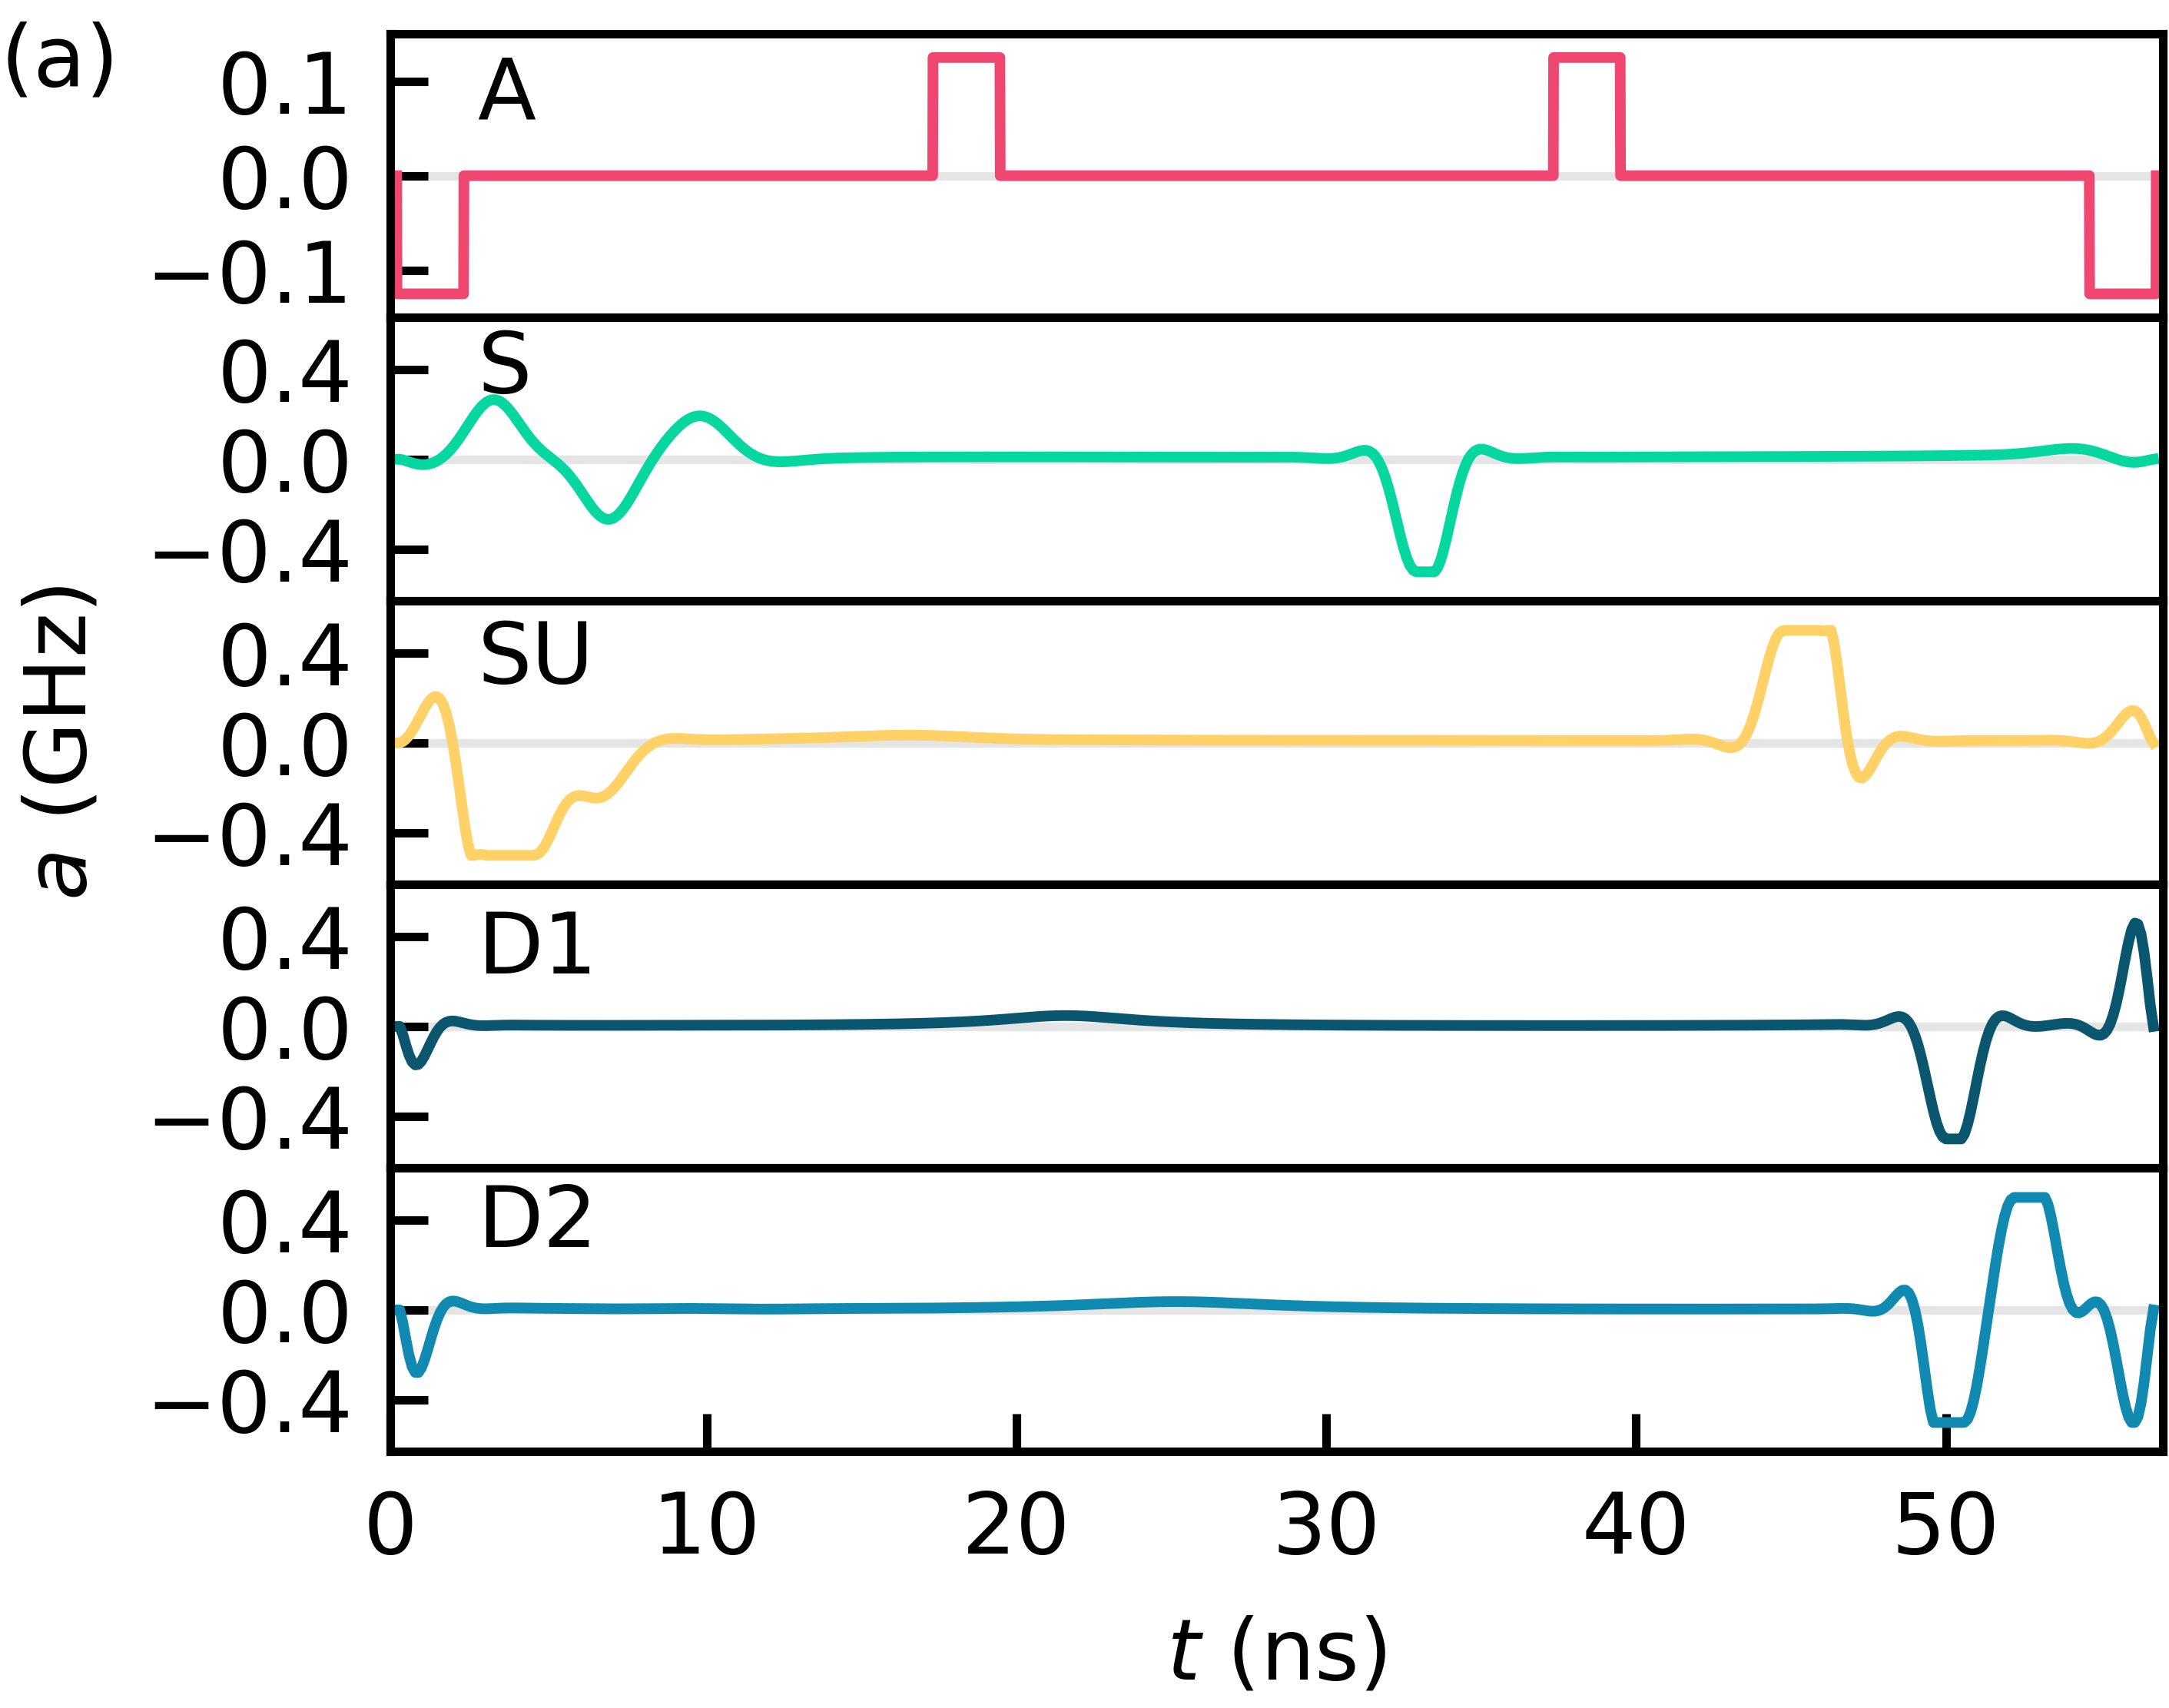
\includegraphics[width=\linewidth]{assets/f3a.png}
  \end{subfigure}\hspace{0.025\textwidth}
  \begin{subfigure}{.4\textwidth}
    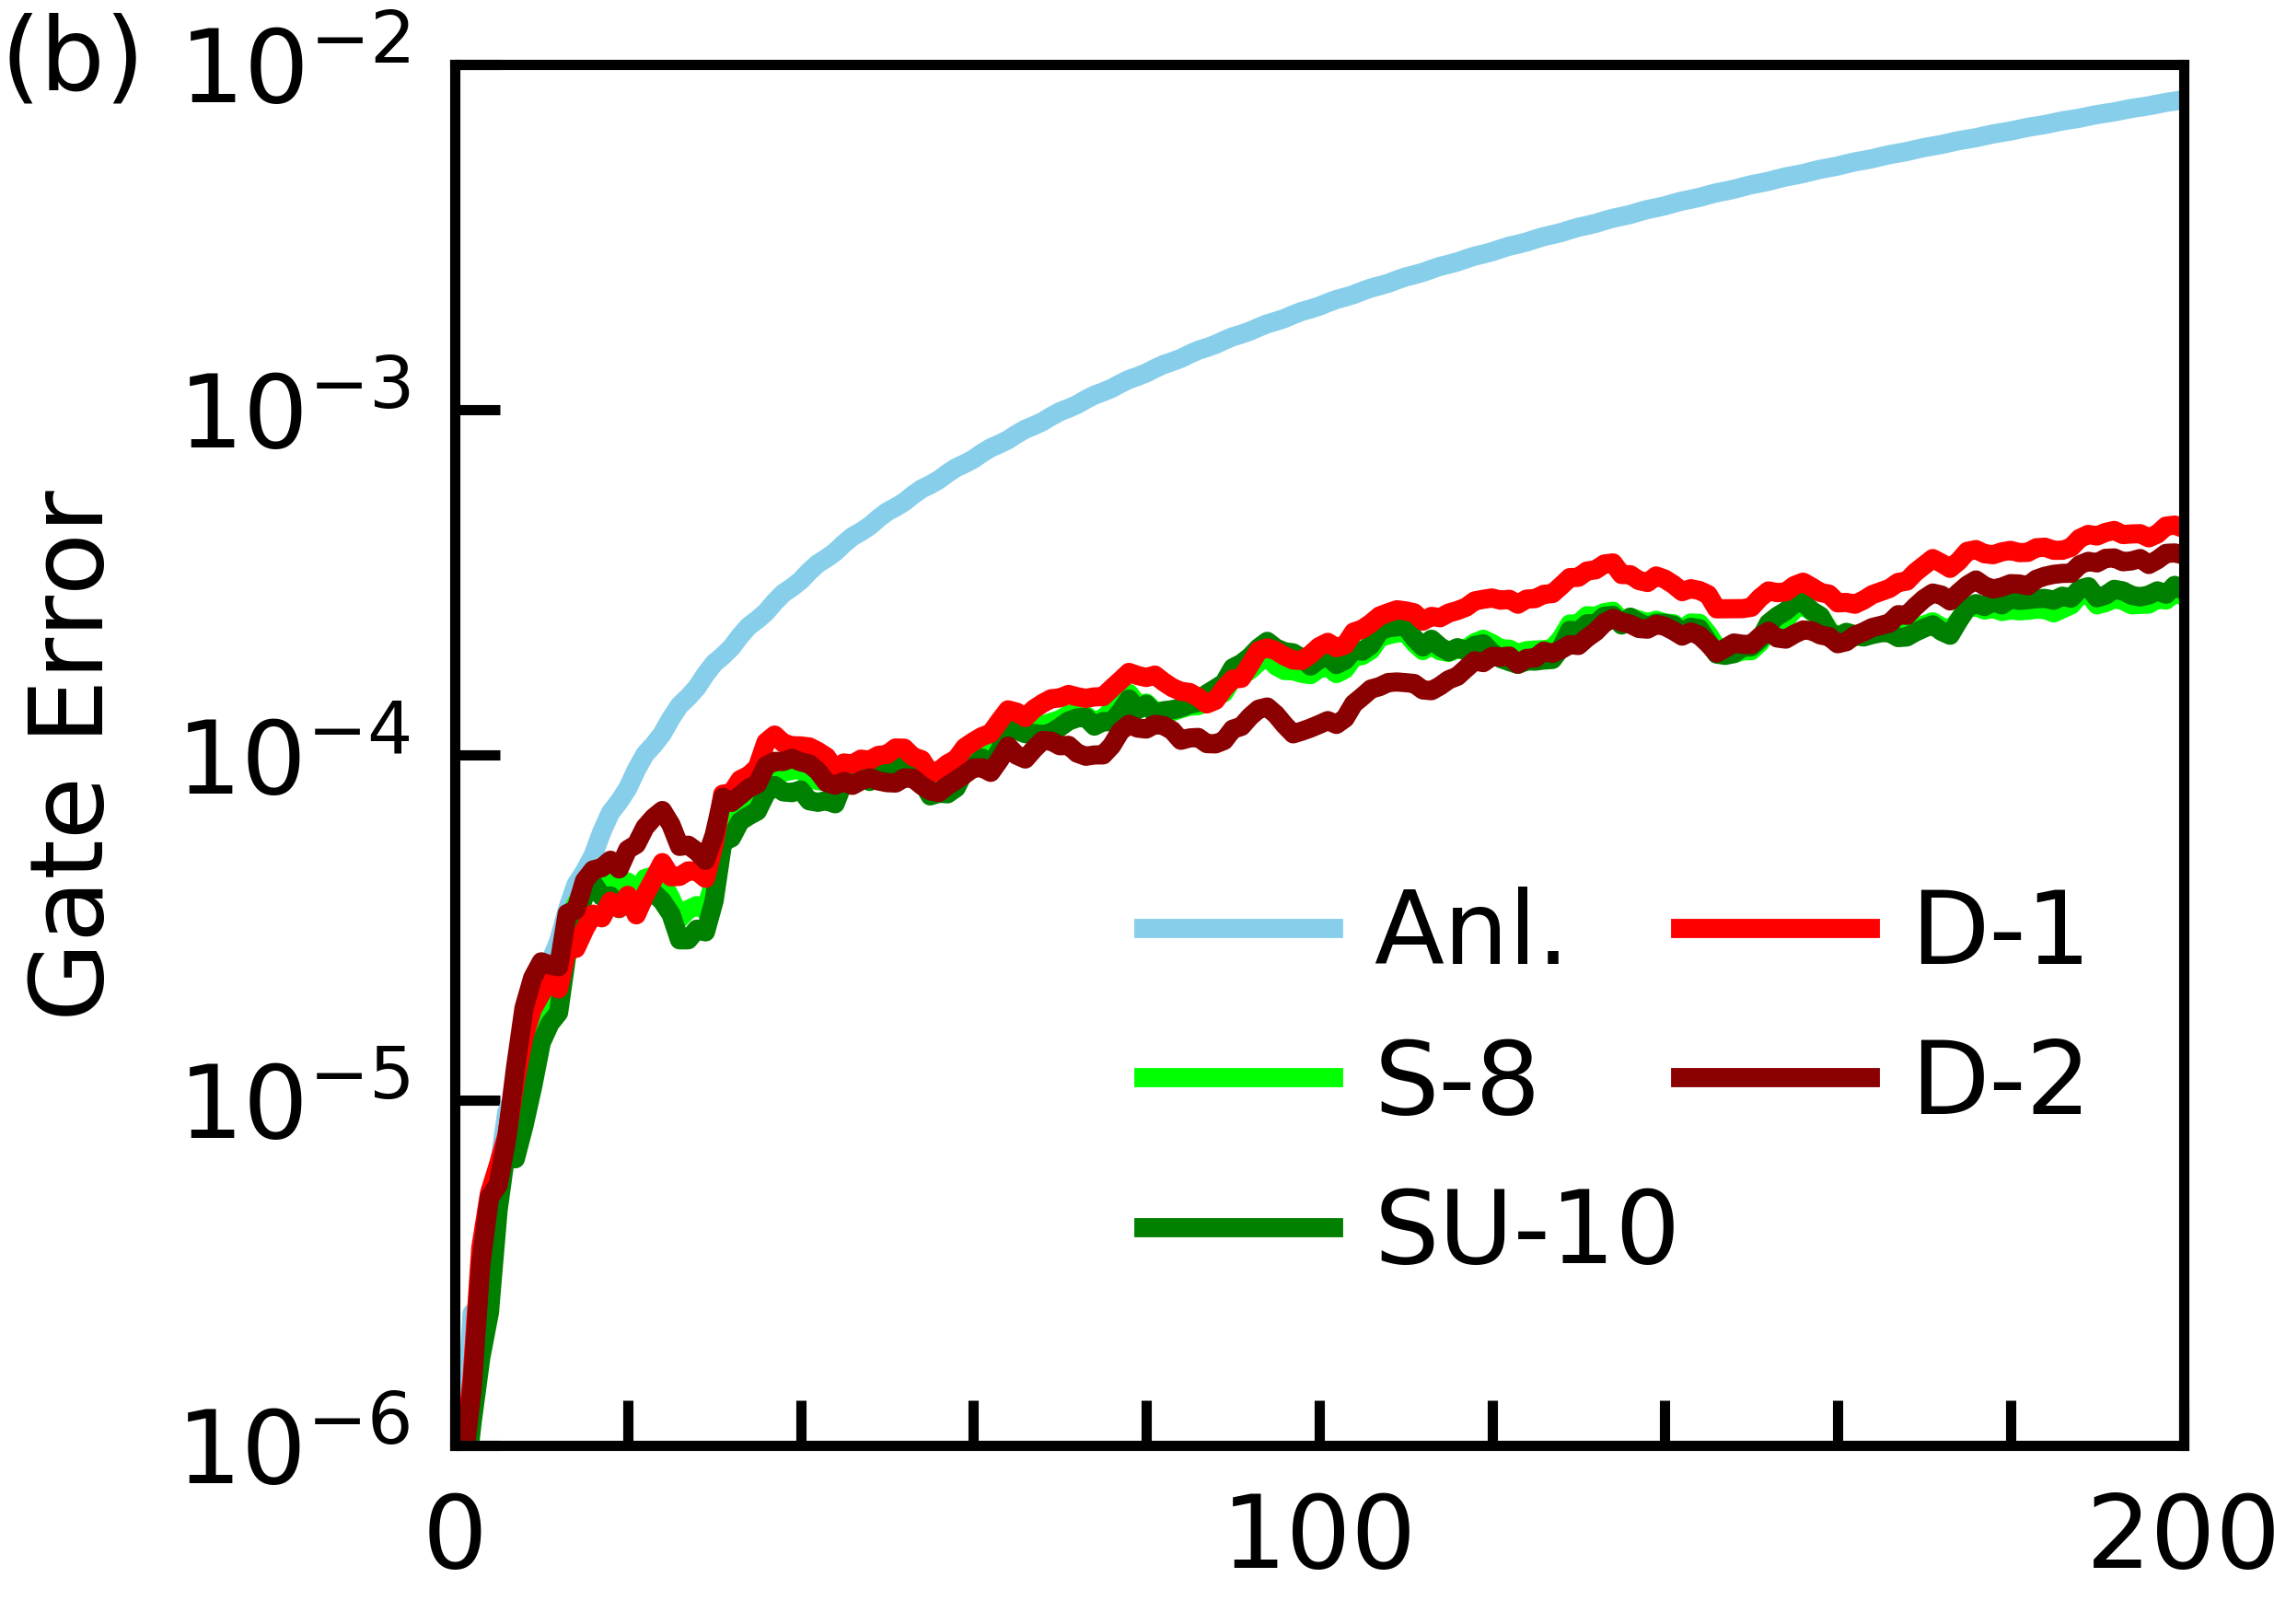
\includegraphics[width=\linewidth]{assets/f3b.png}
  \end{subfigure}
  \caption{
    (a) $X/2$ gates robust to flux offsets constructed with the analytic,
    sampling, unscented sampling, and the 1\textsuperscript{st}-
    and 2\textsuperscript{nd}-order derivative methods. The gates shown
    are the solutions at the analytic gate time.
    (b) Simulation of stochastic 1/$f$ flux noise for
    successive gate applications. The cumulative
    gate error is computed after each gate application.
  }
  \label{fig:stochastic}
\end{figure*}

For the unscented sampling method, $2(2n + d)$ samples
are appended to the augmented state vector \eqref{eq:astatecontrols}
for each initial state from the operator basis. Here $2n = 4$ is the
dimension of the Hilbert space under the isomorphism \eqref{eq:isomorphism}
and $d = 1$ is the number of deviant parameters. The sample
states are used to represent a Gaussian distribution over all $2n$
elements of the initial state, modeling
the uncertainty in the state as a result of the uncertainty in
the deviant parameter. The unscented transformation
is applied to the sample ensemble at each knot point in the discrete dynamics
\eqref{eq:dyn_con} to ensure the first and second moments of the distribution
are accurately propagated. Each sample evolves under the Hamiltonian given in
\eqref{eq:hamiltonian}
where the qubit frequency is replaced by a deviant value determined by the
statistics of the sample ensemble. As in the sampling method,
deviations from the final state are penalized according to \eqref{eq:costfun}.
A detailed update procedure for this method is given
in Appendix \ref{appendix:unscented}.

The derivative method draws on the intuition that
the sensitivity of the state evolution to the deviant parameter
is encoded in the ($l$\textsuperscript{th}-order)
derivative of the state with respect to that parameter
$\partial_{f_{q}}^{l} \psi$.


The $m$\textsuperscript{th}-order
derivative method minimizes the norm of the first $m$
state derivatives with a quadratic cost at each knot point
${\lvert \braket{\partial^{l}_{\lambda} \psi | \partial^{l}_{\lambda} \psi}
  \rvert}^{2}$, $l \in \{1, \dots, m\}$.
The state derivatives could be obtained with backwards mode differentiation.
Naive automatic differentiation would compute
the state derivative at all $1, \dots, k - 1$ knot points
to obtain the state derivative at knot point $k$.
For a single state derivative and $N$ knot points this
requires $O(N^2)$ matrix multiplications.
Instead, we forward propagate the state derivatives in the
augmented state vector under coupled dynamics, resulting in
$O(N)$ matrix multiplications. For example, the dynamics
for the 1\textsuperscript{st}-order derivative method are
\begin{align}
  i \hbar \frac{d}{dt} \ket{\psi} &= H \ket{\psi}\\
  i \hbar \frac{d}{dt} \ket{\partial_{\lambda}\psi} &=
  H \ket{\partial_{\lambda} \psi} +
  (\partial_{\lambda} H) \ket{\psi}
\end{align}
\todo{inconsistent use of $\hbar$ vs $h$.}
Exponential integrators that account for the non-linear
term may be used to efficiently integrate the coupled dynamics,
see Appendix \ref{appendix:derivative}.
\todo{I think this also needs some more explanation. It's not 
clear exactly what you're doing. You're penalizing the derivatives of the dynamics with
respect to the uncertain parameter in the objective, so why do you need to augment the 
state vector? Or are you adding the derivatives to the state vector so that you have 
standard quadratic penalty terms in the objective? Again, I think this confusion would 
be easily cleared up by explicitly writing down your new dynamics, objective function, 
and any additional constraints you impose on the system. Since this is really the meat of 
the paper, it's worth spending the time to make sure this is clear and easy to understand,
especially for those who aren't very familiar with trajectory optimization or optimization 
in general. Also, I think you should explicitly state the size of the problem you're
actually solving. Might be worth putting in a table, along with some timing results, to 
give an idea of how well these methods scale.}

To demonstrate the applicability of these techniques
to mitigate parameter deviations,
we consider the task of achieving a single $Z/2$
gate subject to a constant qubit frequency detuning
$f_{q} \gets f_{q} + \delta f_{q}$.
We take $\sigma_{f_{q}} / f_{q} = 1\%$ to be one standard devation, and equip
the sampling methods accordingly. For each method we compute the gate error for
one simulated gate application subject to the deviant dynamics given by the
stated qubit frequency detuning $\delta f_{q}$.

We compare the numerical methods
to an analytically derived $Z/2$ gate, see Figure \ref{fig:static}a 
\todo{{\LaTeX} suggetion: don't hard-code the sublabels. You can directly reference them.}. 
This gate corresponds to
idling at the flux frustration point $a = 0$. The analytic gate
is at the device's speed limit for a $Z/2$ gate $t_{Z/2} = 1 / 4 f_{q}$ and
is simple to derive. Its erroneous rotation angle $2 \pi t_{Z/2} \delta f_{q}$ is linearly sensitive to
the qubit frequency detuning, resulting in a gate error that is quadratically sensitive
to the qubit frequency detutning.
At a one-percent
qubit frequency detuning the analytic gate achieves a gate error $\sim 4.5 \cdot 10^{-5}$,
which is sufficient for quantum error correction, see Figure \ref{fig:static}b.
Although the analytic $Z/2$ gate performs well, it works
only at the gate time $t_{Z/2}$. The ability to perform $Z$ rotations in arbitrary times is critical
for operating multi-qubit experiments in the lab frame.
Each numerical method is able to find solutions at
all gate times above $t_{Z/2}$, but is unable to find solutions at shorter times.
These numerical methods offer an effective scheme for synchronizing
qubits operating at different frequencies $f_{q, i} \neq f_{q, j}$.

%% TOOD: intro sentence
%% TODO: comment on unscented when it is redone
The sampling and unscented sampling methods
converge on qualitatively similar solutions which combine idling periods
with fast ramps to the maximum amplitude. The gate error at a one-percent
detuning from the nominal qubit frequency achieved
by the sampling method does not improve substantially over the
range of gate durations. The unscented sampling method
achieves linear decreases in its gate error with longer gate durations
until half the larmor period $1 / 2 f_{q}$ after which it achieves a consistent
gate error $\sim 3.5 \cdot 10^{-5}$.
The derivative methods converge on qualitatively similar solutions that
use fast traingle pulses at the boundaries and balance time
on either side of the flux-frustration point symmetrically at low amplitudes.
Both methods achieve a super-linear scaling in their gate error as
a function of the gate duration. The gate error for the 1\textsuperscript{st}-order
derivative method approaches zero at the larmor period $1 / f_{q}$, see Figure \ref{fig:static}c.
We believe the 1\textsuperscript{st}-order method outperforms the 2\textsuperscript{nd}-order
method due to the low contribution of second-order
terms to the gate error in this deviation regime, see Appendix \ref{appendix:derivative}.

Additionally, there are multiple analytic methods 
to mitigate errors due to parameter deviations
including composite pulse sequences \cite{merrill2014progress},
the DRAG scheme \cite{krantz2019quantum}, and
geometric phase considerations
\cite{xu2020nonadiabatic, han2020experimental}.
Composite pulse sequences are derived by computing
the erroneous rotation arising from the parameter deviation
with a finite order magnus expansion.
Pulses are then suitably composed to eliminate the
error. In principle the error may be eliminated
to arbitrary order with sufficiently many pulses \cite{merrill2014progress},
which mirrors the negative correlation between
gate error and gate duration we observe with the derivative method.
It is difficult to choose an appropriate composite pulse
for the problem studied here,
so we propose comparisons between composite pulses and numerical techniques
for future work.
